% Informe IEEE (maximo 5 paginas). Compilar con pdflatex + bibtex (o en Overleaf) desde la carpeta report/.
% Todas las cifras salen de report/tablas_informe.md y de los documentos citados en cada seccion.
\documentclass[conference]{IEEEtran}
\IEEEoverridecommandlockouts
\usepackage[utf8]{inputenc}
\usepackage[T1]{fontenc}
\usepackage[spanish,es-tabla]{babel}
\usepackage{cite}
\usepackage{amsmath,amssymb}
\usepackage{graphicx}
\usepackage{booktabs}
\usepackage{array}
\usepackage{textcomp}
\usepackage{xcolor}
\usepackage{algorithm}
\usepackage{algpseudocode}
\floatname{algorithm}{Algoritmo}
\renewcommand{\algorithmicrequire}{\textbf{Entrada:}}
\renewcommand{\algorithmicfor}{\textbf{para}}
\renewcommand{\algorithmicdo}{\textbf{hacer}}
\renewcommand{\algorithmicend}{\textbf{fin}}
\usepackage{tikz}
\usetikzlibrary{arrows.meta,positioning}
\graphicspath{{./figuras/}}
\usepackage{url}
\usepackage[hidelinks]{hyperref}
\renewcommand{\arraystretch}{0.9}
\setlength{\textfloatsep}{6pt plus 2pt minus 2pt}
\setlength{\floatsep}{6pt plus 2pt minus 2pt}
\setlength{\intextsep}{6pt plus 2pt minus 2pt}
\def\BibTeX{{\rm B\kern-.05em{\sc i\kern-.025em b}\kern-.08em T\kern-.1667em\lower.7ex\hbox{E}\kern-.125em X}}

\renewcommand{\dbltopfraction}{0.92}
\renewcommand{\dblfloatpagefraction}{0.85}
\renewcommand{\textfraction}{0.05}
\setcounter{dbltopnumber}{3}
\begin{document}

\title{Clasificaci\'on de calidad y estimaci\'on de tama\~no de frutas a partir de im\'agenes est\'aticas: el atajo del fondo y la clase \emph{Regular}}

\author{\IEEEauthorblockN{Ximena G\'omez G\'omez, Natalia Delgado, Juan Pablo Bello}
\IEEEauthorblockA{Ingenier\'ia de Sistemas, Universidad Icesi, Cali, Colombia\\
Algoritmos y Programaci\'on III, 2026-2}}

\maketitle

\begin{abstract}
Se construy\'o un sistema que, dada una fotograf\'ia de una fruta (manzana, banano, guayaba, lima, naranja o granada), estima su calidad (Buena, Regular o Mala) y su tama\~no, con una interfaz de carga de imagen o c\'amara. Se compararon una l\'inea base, regresi\'on log\'istica, SVM, Random Forest y una CNN peque\~na desde cero, con partici\'on por objeto f\'isico y un control que solo ve el borde de la imagen. En validaci\'on la mejor fue la CNN (F1 macro 0.725); en la prueba de Kaggle y \emph{Mixed}, usada una sola vez, el SVM (0.774). La advertencia principal es que el rendimiento en Kaggle no demuestra que se aprenda calidad: un modelo que solo ve el borde alcanza un F1 macro de 0.76 a 0.96. En 69 fotos propias ning\'un modelo detecta \emph{Regular} (0 de 14) y el F1 macro de la mejor CNN cae a 0.439.
\end{abstract}

\begin{IEEEkeywords}
clasificaci\'on de frutas, CNN, validaci\'on por grupos, cambio de dominio, \'etica, CRISP-DM
\end{IEEEkeywords}

\section{Introducci\'on}
La clasificaci\'on manual de la calidad de la fruta es lenta, subjetiva y propensa a errores, y las p\'erdidas poscosecha son relevantes: la FAO estima que alrededor del 14\,\% de los alimentos producidos, en valor econ\'omico, se pierde desde la poscosecha hasta el comercio minorista, sin incluirlo \cite{fao2019sofa}.

El objetivo es dise\~nar, entrenar y evaluar un sistema que reciba una imagen est\'atica de una fruta sobre fondo simple y entregue su calidad en tres clases ordenadas y su tama\~no, con carga de imagen y captura con c\'amara. Las contribuciones son: (1) una partici\'on por objeto f\'isico inferido sin identificadores y la medici\'on de la fuga que evita; (2) un control de ``solo borde'' que mide cu\'anto del resultado explica el fondo (con Random Forest en tres clases y tambi\'en con la CNN en dos); (3) la clase \emph{Regular}, inexistente en el dataset base, construida con 760 recortes etiquetados por dos personas; y (4) una evaluaci\'on honesta en 69 fotos propias, usadas una sola vez.

\section{Formulaci\'on del problema}
Sea $x\in[0,1]^{H\times W\times 3}$ una imagen RGB de una fruta de la especie $c\in\{1,\dots,6\}$, con $H=W=96$ para la CNN. La calidad $y\in\{1,2,3\}$ (Buena, Regular, Mala) es \emph{ordinal}, $1<2<3$, y el tama\~no es la longitud normalizada $\ell\in\mathbb{R}_{\ge0}$ de la Ec.~\eqref{eq:ell}. Cada imagen pertenece a un objeto f\'isico $g_i$ y $\mathcal{D}=\{(x_i,c_i,y_i,g_i)\}_{i=1}^{N}$ es el conjunto de datos. Se busca un sistema $x\mapsto(\hat y,\hat\ell)$ que minimice el riesgo esperado
\begin{equation}
R(f)=\mathbb{E}_{(x,y)\sim P}\big[L(f(x),y)\big],
\end{equation}
con $P$ desconocida: se minimiza el riesgo emp\'irico regularizado de la Ec.~\eqref{eq:loss} y $R$ se estima en objetos que el modelo no vio. El sistema debe \emph{generalizar a fotos del equipo}, medido por la brecha $\Delta=\mathrm{F1}_{\text{prueba}}-\mathrm{F1}_{\text{fotos propias}}$.

El problema es complejo por seis razones, cada una evidenciada: (i) \emph{alta dimensionalidad}: $96{\cdot}96{\cdot}3=27\,648$ variables frente a 137 im\'agenes de \emph{Regular} en entrenamiento; (ii) \emph{etiquetas ordinales y ruidosas}: confundir Buena con Mala es m\'as grave que Buena con Regular, y el kappa entre anotadores es 0.607 y 0.606; (iii) \emph{desbalance}: 137 \emph{Regular} frente a m\'as de 10\,000 de las otras clases; (iv) \emph{dependencia entre im\'agenes}: partir por imagen infla el F1 en $\approx 0.027$; (v) \emph{atajos}: el borde de la imagen ya predice la clase; y (vi) \emph{cambio de dominio}: para la CNN T6, $\Delta=0.714-0.439=0.275$. Adem\'as, debe correr en CPU, con 116 ms por foto.

\section{Fundamentos te\'oricos}
\textbf{Clasificaci\'on probabil\'istica.} Un modelo produce logits $z\in\mathbb{R}^K$ y probabilidades $p(k\mid x)=e^{z_k}/\sum_j e^{z_j}$. Se minimiza la entrop\'ia cruzada ponderada con regularizaci\'on L2:
\begin{equation}
\min_\theta\; -\frac1N\sum_{i=1}^{N} w_{y_i}\log p_\theta(y_i\mid x_i)+\lambda\lVert\theta\rVert_2^2,\quad w_k=\frac{N}{K\,N_k}.\label{eq:loss}
\end{equation}
Los pesos $w_k$ compensan el desbalance: el ML tradicional usa $w_k$ y la CNN final, $\sqrt{w_k}$ y sin t\'ermino L2 ($\lambda=0$).

\textbf{Normalizaci\'on.} Los p\'ixeles se escalan a $[0,1]$ (divididos por 255), lo que estabiliza el gradiente. Las caracter\'isticas de color para el ML tradicional (histograma HSV de $8{\times}4{\times}4$ m\'as 8 estad\'isticos, 136 variables) se estandarizan,
\begin{equation}
\tilde z_j=\frac{z_j-\mu_j}{\sigma_j},
\end{equation}
con $\mu_j,\sigma_j$ calculados \emph{solo con entrenamiento}, dentro de un \texttt{Pipeline}, para que la validaci\'on cruzada no filtre estad\'isticos; es imprescindible para el SVM, que usa distancias euclidianas. El aumento de datos se aplica solo en entrenamiento.

\textbf{Modelos.} El SVM RBF resuelve $\min\tfrac12\lVert w\rVert^2+C\sum_i\xi_i$ con $K(x,x')=e^{-\gamma\lVert x-x'\rVert^2}$ \cite{cortes1995svm}; el Random Forest promedia \'arboles que reducen la impureza de Gini $G=1-\sum_k p_k^2$ \cite{breiman2001rf}; ambos con \texttt{scikit-learn} \cite{pedregosa2011sklearn}. Una capa Conv2D con $c_{in}$ canales y $c_{out}$ filtros de $k\times k$ tiene $(k^2c_{in}+1)c_{out}$ par\'ametros y una densa $(n_{in}+1)n_{out}$. Con entrada $128{\times}128{\times}3$ y tres bloques Conv(3$\times$3)+MaxPool de 32, 64 y 128 filtros, la cabeza \texttt{Flatten}+Dense(128) deja 4\,288\,067 par\'ametros y \texttt{GlobalAveragePooling2D} (GAP), 110\,147 (conteos a 128 px verificados contra Keras en las pruebas del repositorio); la CNN final (T6, 96 px) tiene 2\,453\,059 par\'ametros. Se usan Dropout \cite{srivastava2014dropout} y Adam \cite{kingma2014adam}.

\textbf{M\'etricas.} F1 macro (promedio de $F1_k=2P_kR_k/(P_k+R_k)$ sobre las $K$ clases), preferible a la exactitud con desbalance, y el kappa ponderado cuadr\'atico, por ser ordinales las clases \cite{cohen1960kappa,cohen1968weighted},
\begin{equation}
\kappa_w=1-\frac{\sum_{i,j}w_{ij}O_{ij}}{\sum_{i,j}w_{ij}E_{ij}},\qquad w_{ij}=\frac{(i-j)^2}{(K-1)^2}.
\end{equation}
El error est\'andar binomial es $\mathrm{SE}=\sqrt{\hat p(1-\hat p)/n}$; diferencias menores que $2\,\mathrm{SE}$ no se consideran concluyentes.

\textbf{Tama\~no.} Sobre la m\'ascara de la fruta, con $\lambda_1$ el mayor valor propio de la covarianza de sus p\'ixeles, el eje mayor mide $L=4\sqrt{\lambda_1}$ y
\begin{equation}
\ell=\frac{L}{\min(H,W)},\label{eq:ell}
\end{equation}
v\'alida para elipses (eje mayor) y discos (di\'ametro); puede superar 1 en fotos verticales.

\section{Metodolog\'ia}\label{sec:met}
\begin{figure*}[t]
\centering
\begin{tikzpicture}[x=1in,y=1in,
  fase/.style={draw,rounded corners=1pt,minimum width=1.08in,minimum height=0.36in,align=center,font=\scriptsize\bfseries,fill=gray!14},
  det/.style={text width=1.08in,align=left,font=\scriptsize,inner sep=1.5pt},
  flujo/.style={-{Stealth[length=4pt]},thick},
  bucle/.style={-{Stealth[length=4pt]},thick,dashed,red!60!black},
  et/.style={circle,draw=red!60!black,fill=white,inner sep=0.8pt,font=\scriptsize\bfseries,text=red!60!black}]
\foreach \i/\n in {1/{1. Comprensi\'on\\del negocio},2/{2. Comprensi\'on\\de los datos},3/{3. Preparaci\'on\\de los datos},4/{4. Modelado},5/{5. Evaluaci\'on},6/{6. Despliegue}}
  \node[fase] (f\i) at ({(\i-1)*1.19},0) {\n};
\foreach \i/\j in {1/2,2/3,3/4,4/5,5/6} \draw[flujo] (f\i) -- (f\j);
\node[det,below=1pt of f1.south,anchor=north] (t1) {Desperdicio poscosecha; calidad en tres clases y tama\~no.};
\node[det,below=1pt of f2.south,anchor=north] (t2) {19\,526 im\'agenes, 6 especies; \emph{Regular} no existe; solo el borde ya predice la clase.};
\node[det,below=1pt of f3.south,anchor=north] (t3) {Grupos por objeto; 760 recortes de \emph{Mixed} etiquetados; 69 fotos propias.};
\node[det,below=1pt of f4.south,anchor=north] (t4) {L\'inea base, regresi\'on log\'istica, SVM, Random Forest y CNN (Flatten o GAP).};
\node[det,below=1pt of f5.south,anchor=north] (t5) {F1 macro, kappa, error est\'andar y control solo borde; prueba propia de uso \'unico.};
\node[det,below=1pt of f6.south,anchor=north] (t6) {App Streamlit con imagen o c\'amara; calidad, tama\~no y confianza.};
\draw[bucle] (t2.south) -- ++(0,-0.18) -| node[et,pos=0.25]{a} (t3.south);
\draw[bucle] (t5.south) -- ++(0,-0.18) -| node[et,pos=0.25]{b} (t4.south);
\draw[bucle] (t5.south east) -- ++(0,-0.42) -| node[et,pos=0.25]{c} (t3.south east);
\node[font=\scriptsize,text width=6.95in,align=left,anchor=north west,inner sep=0pt] at (-0.54,-1.42) {%
\textbf{\textcolor{red!60!black}{a}} El borde de la imagen ya predice la clase (F1 macro de 0.76 a 0.96): se vuelve a preparaci\'on para partir por objeto y agregar el control solo borde.\\
\textbf{\textcolor{red!60!black}{b}} Con el peso de clase completo la CNN colaps\'o (F1 de validaci\'on 0.30 y 0.32): se vuelve a modelado con un peso suavizado.\\
\textbf{\textcolor{red!60!black}{c}} En fotos propias ning\'un modelo detecta \emph{Regular} (0 de 14): queda como trabajo futuro volver a los datos con m\'as fotos de \emph{Regular} y \emph{Mala}.};
\end{tikzpicture}
\caption{Flujo CRISP-DM del proyecto. Las flechas discontinuas son las iteraciones que ocurrieron y lo que las caus\'o.}
\label{fig:crisp}
\end{figure*}

La Fig.~\ref{fig:crisp} muestra el flujo. \textbf{Negocio:} apoyo a la decisi\'on de calidad y tama\~no. \textbf{Datos:} se usa \emph{Fruit Quality Classification} (Kaggle, CC0) \cite{park_fruit_quality}: 19\,526 im\'agenes de seis especies, 11\,664 \emph{Good}, 6\,788 \emph{Bad} y 1\,074 \emph{Mixed} (varias frutas por foto, sin etiqueta). El an\'alisis exploratorio encontr\'o desbalance (la granada \emph{Good} es el 51\,\% de \emph{Good}), 10 convenciones de nombre, solo 80.3\,\% de nombres con fecha y variabilidad de calidad de imagen: 1\,188 im\'agenes en escala de grises (20.0\,\% de la granada \emph{Good}) y 564 de m\'as de 1\,000 px, todas de esa misma clase.

\textbf{Preparaci\'on.} El dataset no trae identificador de objeto y las im\'agenes del mismo objeto no son independientes. Se infiere el objeto con marcas de tiempo a $\le 3$ s, hash perceptual (aHash de 256 bits) a distancia de Hamming $\le 5$ y, en nombres sin fecha, contador consecutivo con hash a distancia $\le 30$; los grupos son los componentes conexos (3\,360), con umbrales calibrados con datos. La partici\'on usa \texttt{StratifiedGroupKFold} por especie $\times$ calidad (semilla 42). Partir por imagen infla el F1 en $\approx 0.027$ (0.987 frente a 0.960, cota inferior) y el 49.9\,\% de las im\'agenes de prueba tiene un casi-duplicado en entrenamiento; queda fuga residual por rotaciones o recortes.

\textbf{La clase \emph{Regular}} no existe en Kaggle. Se defini\'o por la fracci\'on de superficie con defecto $\rho$: Buena con $\rho<0.10$, Regular con $0.10\le\rho\le0.40$ o un golpe localizado, Mala con $\rho>0.40$, moho o aspecto blando; la madurez no es defecto. De \emph{Mixed} se segmentaron 8\,194 recortes, 3\,978 pasaron los filtros y 760 se etiquetaron por dos personas (dos rondas), con kappa ponderado de 0.607 (360 recortes) y 0.606 (400); los desacuerdos se resolvieron en grupo y resultaron 199 \emph{Regular}. Las etiquetas de Kaggle (\emph{Good}$\to$Buena, \emph{Bad}$\to$Mala) son d\'ebiles. Las 69 fotos propias (34 frutas de cinco especies, con regla) se reservaron como prueba de uso \'unico y se etiquetaron por consenso, sin kappa. Las anotaciones se comparten en el repositorio (\texttt{data/own\_photos/} y \texttt{data/mixed\_labels/}), como pide el enunciado.

\textbf{Modelado.} Se entrenaron una l\'inea base (clase m\'as frecuente), regresi\'on log\'istica, SVM RBF y Random Forest sobre caracter\'isticas de color, con \texttt{GridSearchCV} agrupado ($k=5$, F1 macro), y una CNN desde cero (96$\times$96 px, bloques de 32, 64 y 128 filtros) con cabeza \texttt{Flatten} (T6) o GAP (T7), con pesos de clase suavizados (con el peso completo colaps\'o: F1 de validaci\'on 0.30 y 0.32, frente a 0.725 y 0.623). El entrenamiento se submuestre\'o a $\le 1\,100$ im\'agenes por especie y clase (5\,408 Buena, 137 Regular, 4\,954 Mala). El tama\~no usa la Ec.~\eqref{eq:ell}, tras segmentar la fruta con el umbral de Otsu sobre la saturaci\'on \cite{otsu1979}; la transformada de distancia y \emph{watershed} \cite{vincent1991watershed} se usaron para separar las frutas de \emph{Mixed}. La CNN se implement\'o con TensorFlow \cite{abadi2016tensorflow} y Keras \cite{chollet2015keras}, y la app con Streamlit \cite{streamlit}. El tama\~no se reporta como longitud normalizada; las clases Peque\~no, Mediano y Grande quedan como trabajo futuro. El modelo de la app (CNN T6) se eligi\'o con la validaci\'on, antes de ver la prueba. T\'ecnicas no vistas en clase, declaradas: \texttt{StratifiedGroupKFold}, hash perceptual, componentes conexos, Otsu, \emph{watershed} y Streamlit. El c\'odigo y las anotaciones est\'an en \url{https://github.com/Ximenagg234/fruit-quality-banana} y el video del proyecto, en \url{https://drive.google.com/file/d/1tPYpLZFJcIF8_H9Ii96Xt_JxhAxQ07Hp/view?usp=sharing}. La Tabla~\ref{tab:hp} reporta los hiperparámetros elegidos, el Algoritmo~\ref{alg:pipeline} resume el pipeline y la Tabla~\ref{tab:alt}, las alternativas descartadas.

\textbf{Plan de despliegue.} La app (Streamlit) permite cargar una imagen o capturarla con la c\'amara y muestra calidad, confianza y tama\~no; corre en un computador sin GPU (116 ms por foto) y se ejecuta localmente, sin guardar las im\'agenes. Es un apoyo con revisi\'on humana: si la confianza es menor de 70\,\% se repite la foto y se revisa a mano, igual que ante un resultado \emph{Regular} o una fruta cortada o en la mano. Se propone, sin implementar: (A) recoger fotos del lugar de uso con m\'as \emph{Regular} y \emph{Mala}; (B) reentrenar y exigir que supere a la l\'inea base y al modelo actual en una prueba nueva separada por fruta; (C) un piloto supervisado que registre desacuerdos; (D) publicar con HTTPS o en una Raspberry Pi con c\'amara, revisando la protecci\'on de datos; y (E) monitorear errores y poder volver a la versi\'on anterior.

\begin{table}[t]
\centering
\caption{Hiperparámetros elegidos (F1 macro de validación cruzada agrupada de 5 pliegues en entrenamiento; fuente: {\normalfont\ttfamily 04\_modelado/resultados\_tres\_clases.csv}).}
\label{tab:hp}
\scriptsize
\begin{tabular}{@{}p{1.7cm}p{4.2cm}p{1.2cm}@{}}
\toprule
Modelo & Hiperpar\'ametros & F1 CV \\
\midrule
Log\'istica & $C=10$ & 0.679 \\
SVM RBF & $C=10$, $\gamma=0.003$ & 0.767 \\
Random Forest & 200 \'arboles, sin l\'imite de profundidad, hoja m\'inima de 3 & 0.758 \\
CNN T6 & Flatten, Dropout 0.5, aumento de datos, pesos suavizados; 11 \'epocas corridas, mejor \'epoca 8 & --- \\
CNN T7 & GAP, Dropout 0.5, aumento de datos, pesos suavizados; 8 \'epocas corridas, mejor \'epoca 5 & --- \\
\bottomrule
\end{tabular}
\end{table}

\begin{algorithm}[t]
\caption{Pipeline de entrenamiento, evaluaci\'on y despliegue.}
\label{alg:pipeline}
\scriptsize
\begin{algorithmic}[1]
\Require im\'agenes de Kaggle y \emph{Mixed}; fotos propias
\State inferir el objeto $g_i$ (tiempo, hash, contador); grupos $\leftarrow$ componentes conexos
\State partir con \texttt{StratifiedGroupKFold} por especie $\times$ calidad; reservar las fotos propias como prueba
\State construir \emph{Regular}: etiquetar 760 recortes de \emph{Mixed} entre dos personas y calcular $\kappa_w$
\For{cada modelo (log\'istica, SVM, Random Forest, CNN T6, CNN T7) y el control solo borde (Random Forest)}
  \State normalizar ($\mu_j,\sigma_j$ de entrenamiento en ML tradicional; p\'ixeles$/255$ en la CNN); ajustar (\texttt{GridSearchCV} agrupado o Adam)
  \State evaluar en validaci\'on: F1 macro, $\kappa_w$ y error est\'andar
\EndFor
\State elegir el modelo con la validaci\'on (CNN T6)
\State usar la prueba y las fotos propias \textbf{una sola vez}; reportar F1, recall de \emph{Regular} y $\Delta$
\State desplegar: calidad con la CNN T6 y tama\~no $\ell$ con la Ec.~\eqref{eq:ell}
\end{algorithmic}
\end{algorithm}

\begin{table*}[t]
\centering
\caption{Estrategia de soluci\'on: alternativas consideradas y decisi\'on (detalle en {\normalfont\ttfamily docs/estrategia\_solucion.md}).}
\label{tab:alt}
\scriptsize
\begin{tabular}{@{}p{1.9cm}p{6.6cm}p{8.4cm}@{}}
\toprule
Decisi\'on & Alternativas descartadas y por qu\'e & Elegida y evidencia \\
\midrule
Partici\'on & Aleatoria por imagen (infla el F1 en $\approx 0.027$; 49.9\,\% de la prueba con casi-duplicado); solo marca de tiempo (solo 80.3\,\% de los nombres trae fecha) & Tiempo $\le 3$ s, hash perceptual y contador, con componentes conexos: 3\,360 grupos, calibrados con datos \\
Caracter\'isticas (ML) & P\'ixeles crudos (decenas de miles de variables); HOG o textura (no vistos en clase, no probados) & Histograma HSV y estad\'isticos de color (136 variables): interpretable y barato; hereda el sesgo de fondo \\
Modelos de ML & KNN y XGBoost (no probados: log\'istica, SVM y Random Forest ya cumplen el m\'inimo de dos) & Log\'istica, SVM RBF y Random Forest con \texttt{GridSearchCV} agrupado \\
CNN & Transfer learning con MobileNetV2 \cite{sandler2018mobilenetv2}: explorado solo en validaci\'on (F1 macro 0.760 congelada y 0.717 con ajuste fino, frente a 0.725; no concluyente); se prioriz\'o desde cero; \texttt{Flatten} frente a GAP: 4\,288\,067 frente a 110\,147 par\'ametros a 128 px & CNN desde cero (32-64-128) con las dos cabezas; sin diferencia concluyente en Buena frente a Mala \\
Clase \emph{Regular} & Solo fotos propias (pocas, de un dominio); dataset adicional con nivel intermedio (no descargado); sintetizarla (datos inventados) & 760 recortes de \emph{Mixed} etiquetados por dos personas \\
Desbalance & Pesos completos en la CNN (colaps\'o: F1 de validaci\'on 0.30 y 0.32); SMOTE (no visto, no probado) & Pesos suavizados (ra\'iz cuadrada) en la CNN; completos en el ML tradicional \\
Fotos propias & Repartirlas entre entrenamiento, validaci\'on y prueba (la prueba propia quedar\'ia en 12 fotos) & Solo como prueba final de uso \'unico \\
Tama\~no y despliegue & GrabCut (se extendi\'o a las sombras); $\ell$ dividida por el ancho (cambia con la orientaci\'on); Tkinter, PyQt y Raspberry Pi & Saturaci\'on HSV y Otsu; $\ell$ dividida por $\min(H,W)$; Streamlit \\
\bottomrule
\end{tabular}
\end{table*}

\begin{table*}[t]
\centering
\caption{Decisiones \'eticas (an\'alisis completo en {\normalfont\ttfamily docs/etica\_tabla.md}). Principios de los c\'odigos del IEEE \cite{ieee_policy78} y de la ACM \cite{acm2018code} (numeraci\'on de la ACM, versi\'on 2018).}
\label{tab:etica}
\scriptsize
\begin{tabular}{@{}p{0.3cm}p{4.0cm}p{4.0cm}p{7.6cm}@{}}
\toprule
\# & Situaci\'on o dilema & Principio del c\'odigo & Decisi\'on y evidencia \\
\midrule
E1 & Privacidad: manos, joyas y fondo del hogar en las fotos propias; metadatos GPS & Proteger la privacidad de otros (IEEE); respetar la privacidad (ACM 1.6) & Sin rostros; visto bueno de las personas que salen; fotos reducidas y sin metadatos: 0 de 123 con EXIF o GPS; las fotos no se suben al repositorio. \\
E2 & Consentimiento de terceros en lugares p\'ublicos & Tratar a todas las personas con respeto (IEEE) & Solo frutas propias, sin vendedores ni clientes. \\
E3 & Datos de terceros: procedencia no documentada, posibles casi-duplicados & Acreditar las contribuciones de otros (IEEE); respetar el trabajo de otros (ACM 1.5) & Dataset citado, licencia CC0, sin redistribuir im\'agenes; se declaran los casi-duplicados (49.9\,\% en prueba al partir por imagen). \\
E4 & Sesgos: el fondo delata la clase; \emph{Regular} minoritaria; especies desiguales; etiquetas d\'ebiles & Justicia y evitar da\~nos (IEEE); no discriminar (ACM 1.4) & Partici\'on por objeto; m\'etricas globales y por especie; control de solo borde; doble etiquetado con kappa 0.607 y 0.606. \\
E5 & Honestidad: pocas fotos propias, fuga de datos & Honestidad al afirmar resultados; aceptar cr\'itica (IEEE); ser honesto y digno de confianza (ACM 1.3) & Prueba usada una sola vez; error est\'andar de la exactitud (Tabla~\ref{tab:met}); se reporta lo que falla (0 de 14 \emph{Regular}). \\
E6 & Uso responsable: descartar fruta aprovechable o dejar pasar fruta en mal estado & Seguridad y bienestar del p\'ublico; declarar limitaciones (IEEE); evitar da\~no (ACM 1.2) & Apoyo a la decisi\'on: muestra confianza, avisa si es menor de 70\,\% y que \emph{Regular} es poco fiable; no certifica inocuidad. \\
E7 & Datos de los usuarios de la app & Proteger la privacidad (IEEE); respetar la privacidad (ACM 1.6) & La imagen se procesa en memoria y no se guarda (verificado con una prueba autom\'atica). \\
\bottomrule
\end{tabular}
\end{table*}

\begin{table*}[t]
\centering
\caption{Matriz de impactos y mitigaciones, con la evidencia medida (an\'alisis completo en {\normalfont\ttfamily docs/impactos\_matriz.md}).}
\label{tab:impactos}
\scriptsize
\begin{tabular}{@{}p{1.2cm}p{3.1cm}p{3.5cm}p{3.5cm}p{4.9cm}@{}}
\toprule
Dimensi\'on & Impacto positivo & Riesgo & Mitigaci\'on implementada & Dato medido \\
\midrule
Social & Criterio m\'as uniforme que el manual; herramienta accesible & Sobreconfianza; errores que perjudican especies poco representadas; percepci\'on de vigilancia & Confianza y aviso de baja confianza; alcance declarado; sin guardar im\'agenes & En fotos propias, F1 macro 0.439; 0 de 14 \emph{Regular}; exactitud 0.681 frente a 0.710 de la l\'inea base \\
Econ\'omica & Menos p\'erdidas y desperdicio; bajo costo de adopci\'on & Falsos ``Mala'' (descarte) y falsos ``Buena'' (paso de fruta mala); brecha de adopci\'on & M\'etricas por clase y matrices de confusi\'on; ejecuci\'on local sin servicios de pago & En la prueba, la CNN T6 confunde 73 \emph{Buena} con \emph{Mala} y 54 \emph{Mala} con \emph{Buena} de unas 2\,700 im\'agenes \\
Ambiental & Menos desperdicio de recursos de producci\'on & Consumo de entrenamiento e inferencia & Modelos peque\~nos en CPU; costo informado & 7.2 h de procesos y 0.11 a 0.40 kWh (estimados, no medidos); 116 ms por foto \\
Global & Metodolog\'ia reutilizable con datos locales & Otras variedades, c\'amaras, preferencias de madurez y marcos regulatorios & Alcance y clases con criterios expl\'icitos; sin datos personales & F1 macro de la CNN T6: 0.714 en la prueba de Kaggle y \emph{Mixed}, 0.439 en fotos propias \\
\bottomrule
\end{tabular}
\end{table*}

\begin{figure}[t]
\centering
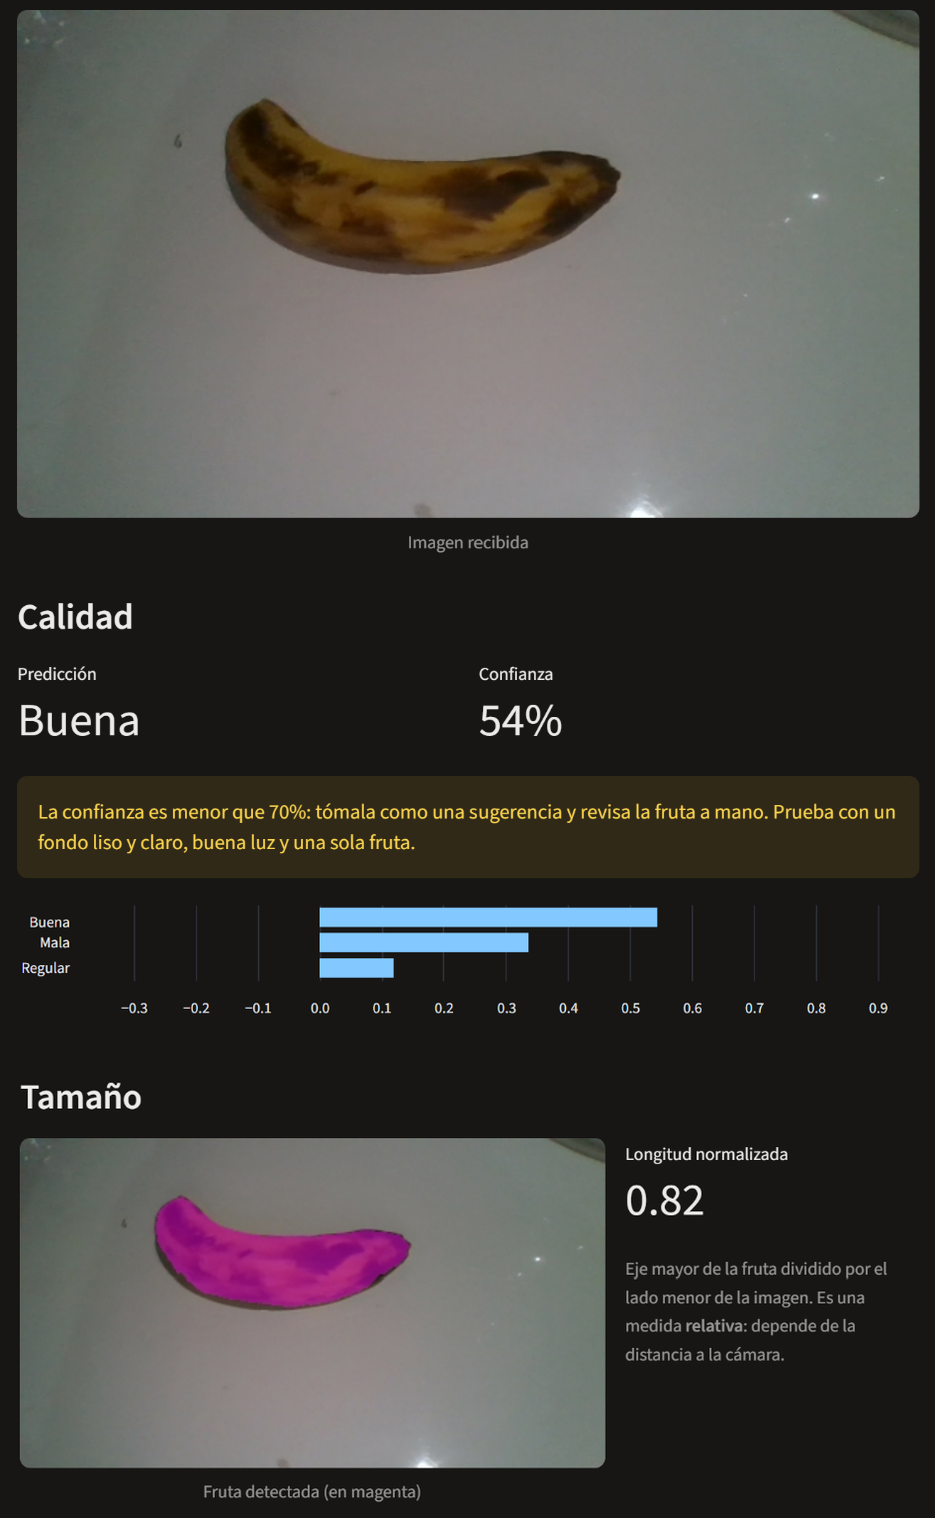
\includegraphics[width=0.72\columnwidth]{app_camara.png}
\caption{App en la prueba con c\'amara: banano con defectos (esperado \emph{Regular}) clasificado como \emph{Buena} con 54\,\% y aviso de baja confianza; abajo, probabilidades, segmentaci\'on y longitud normalizada.}
\label{fig:app}
\end{figure}

\begin{figure}[t]
\centering
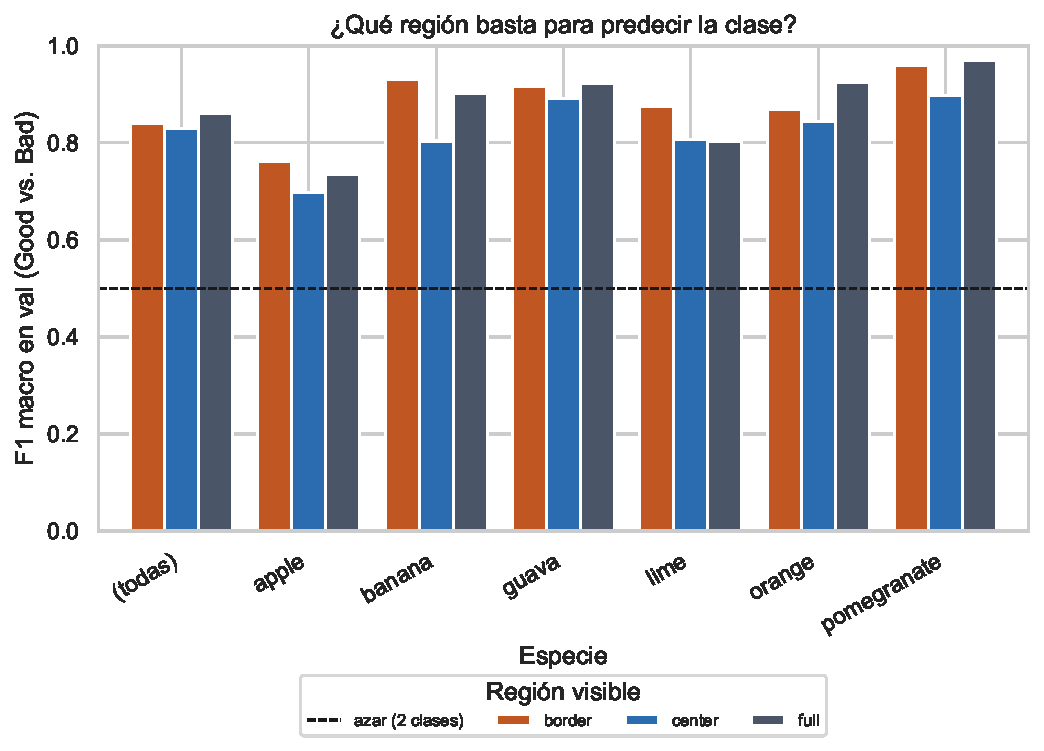
\includegraphics[width=\columnwidth]{prueba_atajo_borde.pdf}
\caption{Prueba del atajo del fondo: F1 macro de un Random Forest que solo ve el borde de la imagen para separar \emph{Good} de \emph{Bad}, por especie.}
\label{fig:atajo}
\end{figure}

\begin{figure}[t]
\centering
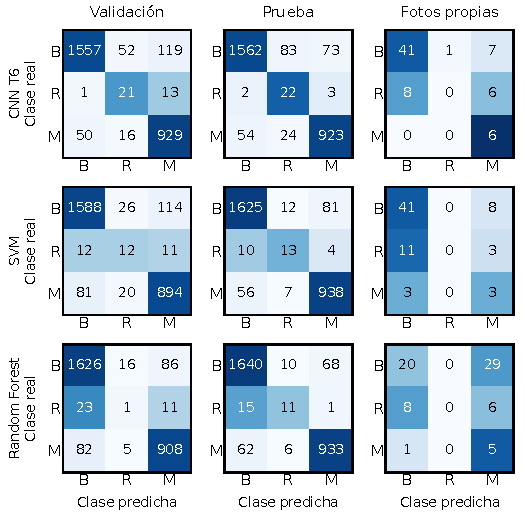
\includegraphics[width=\columnwidth]{matrices_confusion_tres_clases.pdf}
\caption{Matrices de confusi\'on de tres clases (conteos; el color es la proporci\'on de cada clase real). B: \emph{Buena}; R: \emph{Regular}; M: \emph{Mala}.}
\label{fig:conf}
\end{figure}

\begin{figure*}[t]
\centering
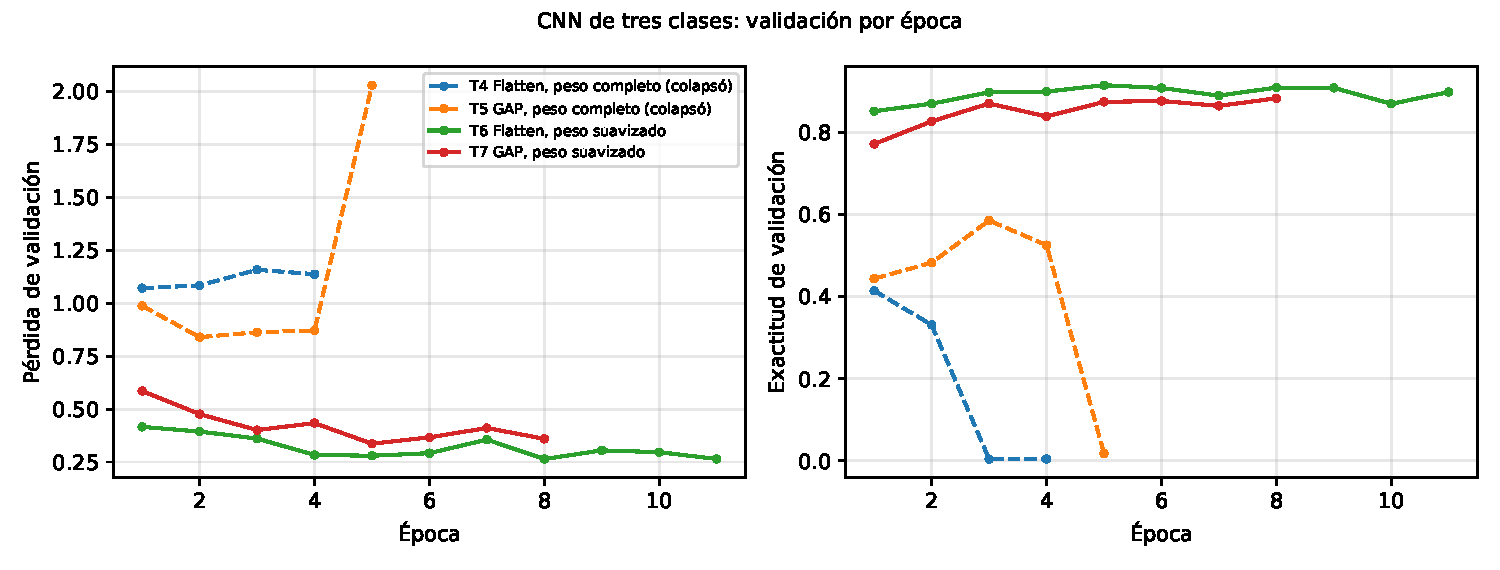
\includegraphics[width=0.74\textwidth]{cnn_curvas_tres_clases.pdf}
\caption{P\'erdida y exactitud de validaci\'on por \'epoca de las CNN de tres clases. T4 y T5 (peso completo) colapsaron; T6 y T7 usan el peso suavizado.}
\label{fig:curvas}
\end{figure*}

\begin{figure*}[t]
\centering
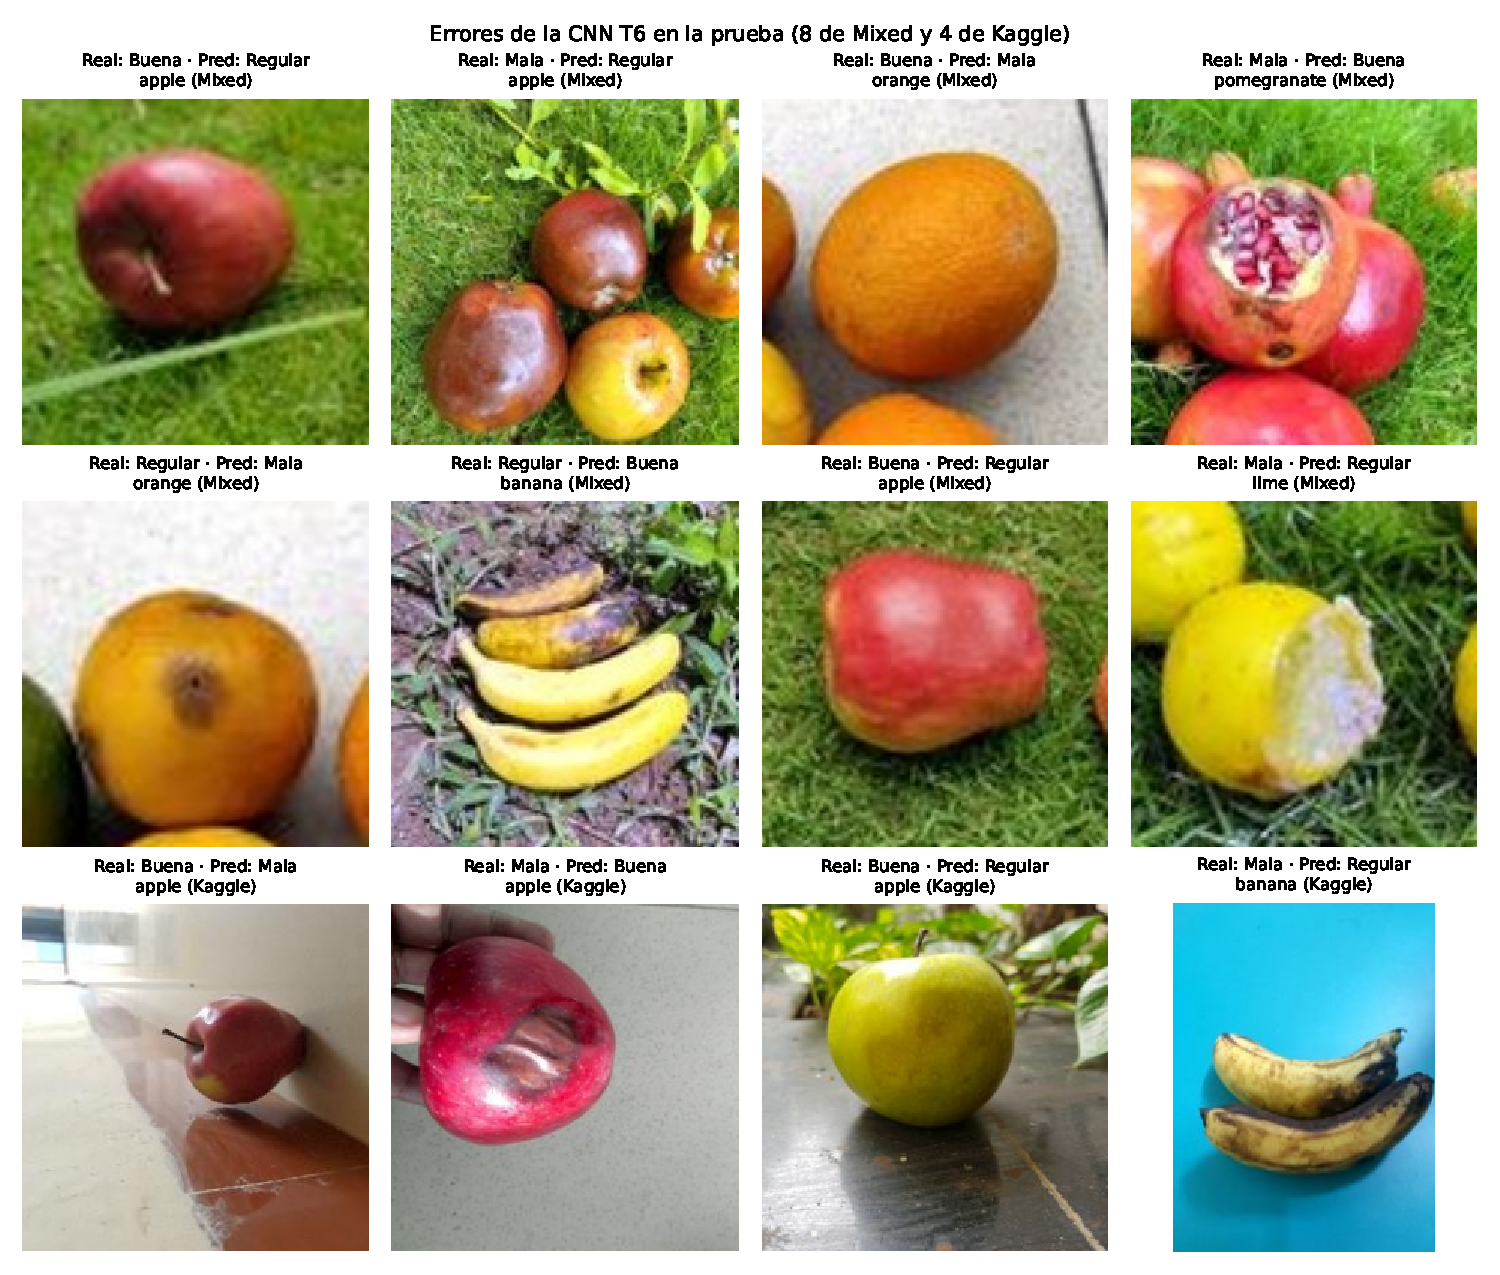
\includegraphics[width=0.6\textwidth]{errores_cnn_T6.pdf}
\caption{Ejemplos de error de la CNN T6 en la prueba (8 de \emph{Mixed} y 4 de Kaggle \cite{park_fruit_quality}).}
\label{fig:errores}
\end{figure*}

\textbf{\'Etica e impactos.} Las Tablas~\ref{tab:etica} y~\ref{tab:impactos} resumen los dilemas, las medidas y los impactos. \emph{Social:} un criterio uniforme reduce la subjetividad de la clasificaci\'on manual, pero la sobreconfianza es un riesgo t\'ecnico real, porque el modelo no detecta \emph{Regular} en fotos propias; por eso la app muestra la confianza, avisa cuando es baja y no guarda im\'agenes (privacidad y percepci\'on de vigilancia). \emph{Econ\'omica:} un falso ``Mala'' descarta fruta aprovechable y un falso ``Buena'' deja pasar fruta en mal estado, as\'i que se reportan los errores por tipo y no solo la exactitud. \emph{Ambiental:} se eligieron modelos peque\~nos en CPU y se informa su costo (7.2 h de procesos y 0.11 a 0.40 kWh estimados). \emph{Global:} las clases se definen con criterios expl\'icitos y el rendimiento debe revalidarse con datos locales, porque el cambio de dominio ya lo degrad\'o. El an\'alisis inicial plane\'o estas mitigaciones y el final comprob\'o cu\'ales se implementaron; quedaron sin lograr m\'as fotos de \emph{Regular} y \emph{Mala}, un piloto con revisi\'on humana y la medici\'on directa de energ\'ia.

\section{Resultados}\label{sec:res}
La Tabla~\ref{tab:res} reporta el F1 macro por modelo y conjunto (l\'inea base: 0.257). En validaci\'on (2\,758 im\'agenes, 35 \emph{Regular}) la CNN T6 es la mejor (0.725, kappa ponderado 0.851, recall de \emph{Regular} 0.60), seguida del SVM (0.693); el Random Forest (0.628) iguala a su control de solo borde (0.630). En la prueba de Kaggle y \emph{Mixed}, usada una sola vez (2\,746 im\'agenes, 27 \emph{Regular}), el SVM (0.774) y el Random Forest (0.765) superan a la CNN T7 (0.736) y a la T6 (0.714); esas diferencias se apoyan en pocos \emph{Regular} y no son concluyentes. En Buena frente a Mala, la mejor CNN alcanz\'o 0.938 (\texttt{Flatten}) y 0.929 (GAP), sin superar al Random Forest (0.947). Como exploraci\'on posterior a la prueba, solo en validaci\'on (35 \emph{Regular}), se entren\'o MobileNetV2 \cite{sandler2018mobilenetv2} (pesos de ImageNet): congelada obtuvo F1 macro 0.760 y recall de \emph{Regular} 0.49 (nuestra CNN: 0.725 y 0.60), y con ajuste fino de las \'ultimas 40 capas, 0.717 y 0.26. La diferencia no es concluyente y la app sigue usando la CNN propia. La Tabla~\ref{tab:met} completa estas cifras con error est\'andar, $\kappa_w$ y \emph{Regular}.

\begin{table}[t]
\centering
\caption{F1 macro por modelo (tres clases). La brecha es entrenamiento menos validaci\'on. Fuente: {\normalfont\ttfamily tablas\_informe.md}, Tabla~5.}
\label{tab:res}
\scriptsize
\begin{tabular}{@{}lccccc@{}}
\toprule
Modelo & Entren. & Valid. & Prueba & Fotos propias & Brecha \\
\midrule
L\'inea base & 0.227 & 0.257 & 0.257 & 0.277 & $-0.03$ \\
Reg. log\'istica & 0.748 & 0.625 & 0.659 & 0.305 & 0.12 \\
SVM (RBF) & 0.929 & 0.693 & 0.774 & 0.363 & 0.24 \\
Random Forest & 0.927 & 0.628 & 0.765 & 0.243 & 0.30 \\
RF solo borde & 1.000 & 0.630 & 0.685 & 0.346 & 0.37 \\
CNN T6 (Flatten) & 0.765 & 0.725 & 0.714 & 0.439 & 0.04 \\
CNN T7 (GAP) & 0.729 & 0.623 & 0.736 & 0.419 & 0.11 \\
\bottomrule
\end{tabular}
\end{table}

\begin{table*}[t]
\centering
\caption{M\'etricas complementarias (tres clases): exactitud $\pm$ error est\'andar, $\kappa_w$ y recall/precisi\'on de \emph{Regular} (--: no predice \emph{Regular}). \emph{Mixed} es el subconjunto de 102 im\'agenes de la prueba; en fotos propias el recall de \emph{Regular} es 0 en todos los modelos. Fuente: {\normalfont\ttfamily 04\_modelado/resultados\_tres\_clases*.csv}.}
\label{tab:met}
\scriptsize
\setlength{\tabcolsep}{3.5pt}
\begin{tabular}{@{}l ccc ccc c cc@{}}
\toprule
 & \multicolumn{3}{c}{Validaci\'on (2\,758)} & \multicolumn{3}{c}{Prueba (2\,746)} & \emph{Mixed} (102) & \multicolumn{2}{c}{Fotos propias (69)} \\
\cmidrule(lr){2-4}\cmidrule(lr){5-7}\cmidrule(lr){8-8}\cmidrule(l){9-10}
Modelo & Exactitud & $\kappa_w$ & R/P & Exactitud & $\kappa_w$ & R/P & Exactitud & Exactitud & $\kappa_w$ \\
\midrule
L\'inea base & 0.627$\pm$0.009 & 0.000 & 0.00/-- & 0.626$\pm$0.009 & 0.000 & 0.00/-- & 0.529$\pm$0.049 & 0.710$\pm$0.055 & 0.000 \\
Reg. log\'istica & 0.844$\pm$0.007 & 0.758 & 0.40/0.09 & 0.871$\pm$0.006 & 0.801 & 0.59/0.12 & 0.461$\pm$0.049 & 0.565$\pm$0.060 & 0.070 \\
SVM (RBF) & 0.904$\pm$0.006 & 0.833 & 0.34/0.21 & 0.938$\pm$0.005 & 0.886 & 0.48/0.41 & 0.588$\pm$0.049 & 0.638$\pm$0.058 & 0.204 \\
Random Forest & 0.919$\pm$0.005 & 0.857 & 0.03/0.05 & 0.941$\pm$0.004 & 0.891 & 0.41/0.41 & 0.539$\pm$0.049 & 0.362$\pm$0.058 & 0.027 \\
RF solo borde & 0.907$\pm$0.006 & 0.829 & 0.06/0.09 & 0.911$\pm$0.005 & 0.828 & 0.19/0.31 & 0.569$\pm$0.049 & 0.638$\pm$0.058 & 0.040 \\
CNN T6 & 0.909$\pm$0.005 & 0.851 & 0.60/0.24 & 0.913$\pm$0.005 & 0.876 & 0.81/0.17 & 0.304$\pm$0.046 & 0.681$\pm$0.056 & 0.498 \\
CNN T7 & 0.874$\pm$0.006 & 0.763 & 0.11/0.12 & 0.905$\pm$0.006 & 0.824 & 0.63/0.28 & 0.441$\pm$0.049 & 0.652$\pm$0.057 & 0.385 \\
\bottomrule
\end{tabular}
\end{table*}

En las 69 fotos propias (49 Buena, 14 Regular, 6 Mala; la l\'inea base de siempre Buena tiene exactitud 0.710) ning\'un modelo detecta \emph{Regular} (0 de 14) y ninguno supera esa exactitud. La mejor es la CNN T6: exactitud $0.681\pm0.056$, F1 macro 0.439, recall de \emph{Buena} 0.84 y de \emph{Mala} 1.00; acierta 0.764 en mano (55 fotos) y 0.357 sobre superficie sin mano (14 fotos), y por especie va de 0.455 (manzana) a 1.000 (lima, 9 fotos). La longitud normalizada correlaciona d\'ebilmente con los cent\'imetros medidos con regla (Spearman 0.26 en 69 fotos; $-0.66$ a $+0.54$ por especie): es una medida relativa. En la prueba con c\'amara (2 casos), un banano con defectos, esperado \emph{Regular}, sali\'o \emph{Buena} con 54\,\% y aviso de baja confianza (Fig.~\ref{fig:app}; \texttt{docs/prueba\_camara.md}).

\section{An\'alisis de resultados}
\textbf{El atajo del fondo.} Con solo el borde (Fig.~\ref{fig:atajo}), el Random Forest separa \emph{Good} de \emph{Bad} con F1 macro de 0.76 (manzana) a 0.96 (granada), y en banano 0.997 con la imagen completa y con solo el borde. Con tres clases el control iguala al modelo completo en validaci\'on (0.630 frente a 0.628). Por eso el rendimiento en Kaggle y \emph{Mixed} no demuestra que se aprenda calidad: la sesi\'on de captura y la clase est\'an asociadas.

\textbf{Generalizaci\'on y sobreajuste.} El F1 macro de la CNN T6 baja de 0.714 a 0.439 en fotos propias: cambio de dominio (manos, fondos, otras frutas y c\'amara). El Random Forest llega a 0.243 y llama \emph{Mala} a 29 de las 49 \emph{Buena}, compatible con que use el fondo como pista (hip\'otesis, no probada). Seg\'un la brecha de la Tabla~\ref{tab:res}, el Random Forest ($0.30$) y el SVM ($0.24$) memorizan el entrenamiento, mientras que la CNN T6 casi no se sobreajusta ($0.04$); sin embargo, esa brecha peque\~na no evita la ca\'ida en fotos propias, que se asocia m\'as bien al cambio de dominio. La Fig.~\ref{fig:curvas} muestra las curvas por \'epoca: con el peso completo (T4, T5) la validaci\'on colaps\'o y con el suavizado (T6, T7) se mantuvo estable.

\textbf{Qu\'e falla.} \emph{Regular} es la clase d\'ebil. Seg\'un las matrices de la Fig.~\ref{fig:conf}, en validaci\'on la T6 acierta 21 de 35 pero llama \emph{Regular} a 68 im\'agenes que no lo son (precisi\'on 0.24); en la prueba acierta 22 de 27 con 107 falsas alarmas (precisi\'on 0.17). El desacuerdo entre anotadores (kappa 0.607 y 0.606) se concentr\'o en el l\'imite \emph{Regular}/\emph{Mala}: la frontera es dif\'icil incluso para las personas, lo que limita lo que un modelo puede aprender. Los ejemplos de error (Fig.~\ref{fig:errores}) muestran manchas peque\~nas u otras frutas en el recorte. El punto m\'as d\'ebil de la T6 es \emph{Mixed}: exactitud $0.30\pm0.05$, por debajo de la l\'inea base ($0.53\pm0.05$) y del SVM ($0.59\pm0.05$), con recall de \emph{Regular} 0.81 pero de \emph{Buena} 0.09 (Tabla~\ref{tab:met}); su F1 global en la prueba se apoya en las im\'agenes de Kaggle.

\textbf{Literatura.} Geirhos et al. \cite{geirhos2020shortcut} definen un atajo como una regla que rinde bien con datos de la misma distribuci\'on pero falla fuera de ella, y recomiendan pruebas fuera de distribuci\'on: nuestras fotos propias lo son, y all\'i el F1 macro cae de 0.714 a 0.439. Xiao et al. \cite{xiao2020noise} muestran que modelos que solo ven el fondo alcanzan 40 a 50\,\% de exactitud en ImageNet-9 (azar: 11\,\%), an\'alogo a nuestro 0.76 a 0.96 con solo el borde. Barz y Denzler \cite{barz2020purging} hallan que 3.3\,\% y 10\,\% de las im\'agenes de prueba de CIFAR-10 y CIFAR-100 tienen duplicados en entrenamiento; en nuestro dataset, al partir por imagen, es el 49.9\,\%. En frutas, Palakodati et al. \cite{palakodati2020fresh} reportan 97.82\,\% de exactitud con una CNN de tres capas convolucionales en tres frutas de Kaggle (5\,989 im\'agenes) y Bird et al. \cite{bird2022fruit}, 83.77\,\% con VGG16 en limones sanos y no sanos (2\,690 im\'agenes), que sube a 88.75\,\% con im\'agenes sint\'eticas; ninguno discute casi-duplicados ni reporta un control de solo borde. Knott et al. \cite{knott2023facilitated} obtienen 0.950 de exactitud en manzana (la mejor CNN, 0.958) con caracter\'isticas DINO y clasificadores cl\'asicos, y atribuyen parte del solapamiento entre clases de madurez del banano a ruido de etiquetas, como nuestro kappa de 0.6. Nuestro Buena frente a Mala (F1 macro 0.938 en validaci\'on) es de magnitud comparable, con m\'etricas y datos distintos; a la luz de estos trabajos, una exactitud alta no prueba por s\'i sola que se aprenda calidad.

\textbf{Limitaciones.} Las fotos propias se etiquetaron por consenso (sin kappa); hay pocos \emph{Regular} en validaci\'on (35), prueba (27) y fotos propias (14); la energ\'ia es una estimaci\'on, no una medici\'on.

\section{Conclusiones y trabajo futuro}
\begin{enumerate}
\item Se construy\'o un pipeline completo (datos, partici\'on por objeto, tres clases, modelos cl\'asicos, CNN y app con c\'amara) (Fig.~\ref{fig:crisp}): F1 macro de 0.725 en validaci\'on con la CNN T6 (l\'inea base 0.257) y de 0.774 en la prueba de Kaggle y \emph{Mixed} con el SVM (Tabla~\ref{tab:res}).
\item Se midi\'o el atajo del fondo: el control de solo borde alcanza 0.76 a 0.96 (Fig.~\ref{fig:atajo}) e iguala al Random Forest completo en validaci\'on (Tabla~\ref{tab:res}); por eso cada resultado lleva su control.
\item Se construy\'o la clase \emph{Regular} con 760 recortes (kappa 0.607 y 0.606) (Sec.~\ref{sec:met}). Es la m\'as dif\'icil: en fotos propias ning\'un modelo la detecta (0 de 14) (Fig.~\ref{fig:conf}).
\item El l\'imite principal es la generalizaci\'on a fotos propias: el F1 macro de la mejor CNN baja de 0.714 a 0.439; la CNN T6 es la que menos se sobreajusta (brecha 0.04) (Tabla~\ref{tab:res}) y acierta las 6 \emph{Mala} (Fig.~\ref{fig:conf}). El tama\~no es relativo (Spearman 0.26) (Sec.~\ref{sec:res}).
\item El sistema es un apoyo a la decisi\'on, no un control de inocuidad (Tabla~\ref{tab:etica}, E6; Tabla~\ref{tab:impactos}).
\end{enumerate}
\textbf{Trabajo futuro, derivado de los errores medidos} (Fig.~\ref{fig:conf}; Tabla~\ref{tab:res})\textbf{:} m\'as fotos propias de \emph{Regular} y \emph{Mala} sobre superficie y sin mano, y entrenar con parte de ellas; sobremuestrear \emph{Regular}; evaluar el transfer learning con una prueba nueva; un dataset con nivel intermedio; un umbral de decisi\'on conservador; y probar otras c\'amaras e iluminaci\'on.

\bibliographystyle{IEEEtran}
\bibliography{refs}

\end{document}
